
Die heutigen Netzwerke, vorallem von kleineren Firmen, basieren vielfach noch auf IPv4\index{IPv4}\footnote{\label{foot:theorie-ipv4}IPv6\index{IPv6} ist in den Startl\"ochern, kann jedoch noch nicht bei jedem Dienstleister genutzt werden.} mit einem stark begrenzten Adressraum\footnote{\label{fot:theorie-piv4-numbers}IPv4 hat einen Adressraum von $2^{32}$ Adressen, IPv6 hingegen $2^{128}$. IPv6 ist also um den Faktor $2^{96}$ gr\"osser und bietet viele Vereinfachungen auf Protokoll- und auf Sicherheitsebene.}. Dies hat den Grund, dass die Internet Service Provider (ISP) ihre Angebote (oder oder Technik) vielfach noch nicht auf den IPv6-Standard aktualisiert haben, da sie noch \"uber eine gen\"ugend grosse Anzahl an IPv4-Adressen verf\"ugen\footnote{Dieser Fakt wird sich in den kommenden Monaten wahrscheinlich \"andern, da seit dem 1. Februar 2011 die restlichen verf\"ugbaren \/8-er Bl\"ocke auf die f\"unf regionalen Internet Registries (RIRs) verteilt worden sind: \url{http://www.apnic.net/publications/news/2011/delegation}. Es k\"onnen somit nur noch wenige tausend IPv4-Adressen bei den den RIRs angefordert werden.}. Das hat zur Folge, dass Server welche nur innerhalb einer Firma genutzt werden, in einem privaten Netzwerk stehen und durch NAT\footnote{\label{foot:theorie-nat}Eine NAT basierende Firewall kann so konfiguriert werden, dass nur eine Anfrage an Port 80 an einen bestimmten Server innerhalb des Netzwerkes weitergeleitet wird, nicht jedoch eine Anfrage auf einem anderen Port.}-Regeln\index{NAT} abgeschirmt sind. Eine Firma hat somit meistens nur eine \"offentliche IP-Adresse, kann durch eine NAT-Firewall aber verschiedene Dienste von unterschiedlichen internen Servern \"offentlich anbieten. Es k\"onnen aber auch Systeme im Netzwerk existieren, welche IP-Technisch komplett vom Internet abgeschirmt sind, da sie aus dem Internet nicht erreichbar sind. Ein \"Uberwachungssystem soll aber nicht nur die eine \"offentliche IP-Adresse pr\"ufen, sondern auch in der Lage sein, alle weiteren nicht \"offentlich zug\"anglichen Server und Dienste zu pr\"ufen. Diese Problematik wird in Kapitel \ref{sec:theorie-nat} behandelt. Auf die grundlegende Problematik von IPv4 und IPv6 basierenden Netzwerken sowie die verschiedenen NAT-Techniken und -Prinzipien wird in dieser Arbeit nicht eingegangen. Dar\"uber existieren nicht nur viele Berichte im Internet sondern auch diverse Artikel in Fachzeitschriften und B\"uchern, wie Beispielsweise "`Computernetzwerke von Andrew S. Tannenbaum \cite{tannenbaum}"'.

Ein weiterer Schwerpunkt liegt in der Definierung von Ger\"aten in einem Netzwerk. Systeme sollten nicht nur manuell in einer Liste eingetragen, sondern auch automatisch aufgefunden werden k\"onnen. Dies nicht nur im aktuellen, lokalen Netzwerk, sondern auch in einem entfernten, welches ebenfalls \"uberwacht wird. Das Auto-Discovery, auch Host-Discovery genannt, muss nicht nur erkennen k\"onnen, ob auf einem gefundenen System eine Instanz der \"Uberwachungs-Software l\"auft, sondern auch, ob dies ein einfach zu \"uberwachendes oder sogar ein zu ignorierendes Ger\"at darstellt.

Sind alle Ger\"ate aus dem aktuellen und allen anderen Netzwerken bekannt, m\"ussen diese anschliessend automatisch fragmentiert werden. Es muss also bestimmt werden, welche Systeme welche Komponenten und Dienste aus dem internen und aus entfernten Netzwerken \"uberwachen, wo die Konfiguration gespeichert wird und wie diese aufgeteilt ist, was beim auffinden eines Problems passiert und wie dieses gemeldet werden kann, sowie was f\"ur Techniken es zur System\"uberwachung und Daten\"ubermittlung gibt. Bei der \"Ubermittlung von Problemen, also dem senden einer Alert-Meldung\footnote{Eine Alert-Meldung ist eine Alarmierungs-Nachricht.}, muss besonders beachtet werden, dass ein und das selbe Problem nicht mehrmals von verschiedenen \"Uberwachungsservern gesendet wird.

%%%%%%%%%%%%%%%%%%%%%%%%%%%%%%%%%%%%%%%%%%%%%%%%%%%%%%%%%%%%%%%%%%%%%%%%%%%%%%%%%%%%%%%%%%%%%%%%%%%%%%%%%%%%%%%%%%%%%%%%%%%%%%%%%%%%%%%%%

\section{Problemfall NAT} \label{sec:theorie-nat} \index{NAT}
Sollen Server innerhalb eines durch NAT abgeschirmten Netzwerkes \"uberwacht werden, m\"usste f\"ur jeden Server eine NAT-Regel definiert werden, damit dieser nicht nur intern, sondern auch von extern erreichbar und somit \"uberwachbar ist. Wenn nun mehrere Dienste, zum Beispiel HTTP\cite{rfc1945}\cite{rfc2616}\index{HTTP}, SMTP\cite{rfc5321}\index{SMTP}, POP3\cite{rfc1939}\index{POP3}, IMAP\cite{rfc3501}\index{IMAP}, ICMP\cite{rfc792}\index{ICMP} und FTP\cite{rfc959}\index{FTP}, auf einem Server \"uberwacht werden sollen, m\"usste nicht nur eine NAT-Regel definiert werden sondern deren sechs. Je mehr Server und Dienste also in einem abgeschirmten Netzwerk von ausserhalb erreichbar sein sollen, desto mehr NAT-Regeln m\"ussen erstellt werden. Die Anzahl kann durch
\begin{equation}
R = \sum_{H=1}^{M} {S_H}
\label{eq:theorie-nat}
\end{equation}
berechnet werden, wobei $R$ die Anzahl der NAT-Regeln, $M$ die Anzahl Server, $H$ der aktuelle Server und $S_H$ die Anzahl Dienste auf diesem beschreiben.

Die Problematik bei den erstellten NAT-Regeln\index{NAT-Regel} liegt nicht nur bei der begrenzten Anzahl an Ports\footnote{\label{foot:theorie-ports}TCP/IP und UDP verf\"ugen \"uber jeweils 65535 Ports} bei TCP\cite{rfc675}\index{TCP} und UDP\cite{rfc768}\index{UDP} basierenden Protokollen, sondern diese Regeln stellen ein erhebliches Sicherheitsrisiko dar. Alle Systeme welche Anfragen an die NAT-Firewall stellen k\"onnen, in den meisten Szenarien wahrscheinlich das gesamte Internet, sind nun ebenfalls in der Lage die verschiedenen Dienste auf den internen Servern nutzen.

\subsection{Source basierende NAT-Regeln} \label{sec:theorie-nat-src} \index{NAT-Regel}
Eine M\"oglichkeit dieses Problem zu beseitigen w\"are, die NAT-Regeln nicht nur an den Port und das Protokoll zu binden, sondern auch auf den Source-Host\footnote{\label{foot:theorie-sourcehost}Der Source-Host ist ein System, welches eine Anfrage startet. Der Destination-Host ist das System, an welches die Anfrage gerichtet wird}\index{Source-Host}\index{Destination-Host}. Somit m\"usste nicht nur eine Regel pro Host und Dienst erstellt werden, sondern zus\"atzlich noch eine f\"ur jeden Source-Host in allen entfernten Netzwerken, welche ebenfalls in das \"Uberwachungsnetzwerk eingeschlossen sind (siehe Abbildung \ref{fig:nat-source} im Anhang). Die Anzahl der ben\"otigten Regeln kann durch eine Multiplikation der Anzahl Dienste mit der Anzahl Source-Hosts berechnet werden. Das wird durch die Formel
\begin{equation}
 R = \sum_{H=1}^{M} {S_H \times N}
\label{eq:theorie-nat-sec}
\end{equation}
wiedergegeben, wobei $N$ die Anzahl an Rechnern ist, welche eine Verbindung aufbauen k\"onnen m\"ussen.

Die Anzahl Regeln w\"urde sich also bei jedem neuen Host oder Dienst vervielfachen, wie Tabelle \ref{tbl:theorie-nat} zeigt. Auch m\"usste jede NAT-Firewall im gesamten \"Uberwachungs-Netzwerk neu konfiguriert und eingestellt werden.

\begin{table}[ht]
\centering
\begin{tabular}{ccc}
 \toprule
 Anzahl Dienste & Anzahl entfernte Hosts & Anzahl NAT-Regeln\\
 \midrule
 10 & 1 & 10\\
 10 & 2 & 20\\
 10 & 5 & 50\\
 10 & 20 & 200\\
 10 & 21 & 210\\
 10 & 50 & 500\\
 10 & 51 & 510\\
 \bottomrule
\end{tabular}
\caption[Anzahl NAT-Regeln bei vielen Diensten]{Anzahl NAT-Regeln bei gleich bleibender Anzahl zu \"uberwachenden Dienste und steigender Anzahl von Hosts, welche diese Dienste \"uberwachen}
\label{tbl:theorie-nat}
\end{table}


\subsection{Umgehung der NAT-Problematik} \label{sec:theorie-nat-fazit}
Um die NAT-Regeln und den damit zugrunde liegenden Aufwand zu verringern, w\"are eine M\"oglichkeit, dass alle Netzwerke in sich ein geschlossenes System bilden. Die Systeme in einem Netzwerk \"uberwachen also alle Dienste und Komponenten ihres eigenen Netzwerkes. Um die Erreichbarkeit der einzelnen Netzwerke zu \"uberwachen, werden diese in der Theorie ebenfalls als einzelne Systeme angeschaut, welche sich gegenseitig \"uberwachen (siehe Abbildung \ref{fig:nat-verteilt} im Anhang). Es werden also zwei verschiedene "`\"Uberwachungsnetzwerke"' definiert: Die einzelnen Komponenten innerhalb eines Netzwerkes \"uberwachen sich gegenseitig; Die verschiedenen Netzwerke werden als einzelne Systeme angesehen und \"uberwachen sich gegenseitig.

Die \"Uberwachung von \"offentlichen Diensten wie Web und EMail stellt dabei kein grosses Problem dar, denn diese sind wahrscheinlich von \"uberall her erreichbar und somit auch \"uberwachbar. Die interessantere Frage in diesem Kontext ist vielmehr, wie man trotz Firewalls pr\"ufen kann, ob ein Netzwerk verf\"ugbar/erreichbar ist oder nicht.

\subsubsection{ICMP-Pakete} \label{sec:theorie-nat-fazit-icmp} \index{ICMP}
ICMP\cite{rfc792}\footnote{Mit ICMP oder auch PING wird umgangssprachlich ein ECHO-Request in einem IPv4 oder IPv6 Netzwerk betitelt.} zeichnet sich durch sehr kleine und einfache Pakete aus, welche alle notwendigen Informationen zur Bestimmung von Latenzen sowie der Erreichbarkeit eines Systems beinhalten. Viele \"Uberwachungs-Tools setzen aus diesem Grund auch ICMP f\"ur diese Zwecke ein. Der Nachteil ist, dass diese Pakete vielfach von Firewalls geblockt oder als unzustellbar zur\"uckgeschickt werden\footnote{\label{foot:theorie-verteilt-icmp}Die Ablehnung von ICMP-Paketen macht zum Beispiel Sinn, wenn man nicht will, dass andere auf eine schnelle Art und Weise herausfinden k\"onnen, dass etwas da ist. Ein Portscan (auffinden eines offenen Ports bei einem System) dauert einiges l\"anger und wird von den meisten Firewalls erkannt und somit ebenfalls geblockt}. Dies kann jedoch umgangen werden, indem pro Netzwerk eine Regel definiert wird, welche ICMP zulassen w\"urde.

Eine ICMP-Pr\"ufung kann nur gew\"ahrleisten, dass der Router (respektive der Gateway) des entfernten Netzwerkes augenscheinlich vorhanden ist und auf den ECHO-Request Antworten kann. Es k\"onnen weder Daten noch Statusmeldungen etc. \"uber dieses Protokoll ausgetauscht werden.

\subsubsection{\"Uberwachungs-Agenten} \label{sec:theorie-nat-fazit-proxy}
Eine andere M\"oglichkeit um Pr\"ufungen zwischen verschiedenen Netzwerken zu realisieren sind spezielle Proxies, respektive Agenten. Ein Agent kann eine Nachricht empfangen, an ein System weiterleiten und gegebenenfalls dessen Antwort wieder zur\"ucksenden.

Die Problematik bei einem einzelnen Agenten pro Netzwerk ist jedoch, dass wenn dieser nicht l\"auft, es den Anschein macht, dass das komplette Netzwerk nicht online ist. F\"ur diesen Fall, also wenn ein Proxy keine Antwort sendet, k\"onnte die ICMP-L\"osung (siehe Kapitel \ref{sec:theorie-nat-fazit-icmp}) als Fallback-L\"osung\footnote{Bei ICMP als Fallback-L\"osung kommt wieder das Problem zum tragen, dass ECHO-Requests vielfach auf den Firewalls geblockt/abgewiesen werden} eingesetzt werden. Dadurch weiss man anschliessend jedoch nur, ob wirklich das Netzwerk oder einfach nur der Agent nicht online ist.

Eine weitaus bessere M\"oglichkeit als der ICMP-Fallback ist es, pro Netzwerk mehrere Agenten zu definieren. Wenn von einem Agenten keine Antwort kommt, kann der zweite und dritte Agent noch gepr\"uft werden. Wenn keiner der Agenten eine Antwort gibt, kann mit einer gewissen Wahrscheinlichkeit davon ausgegangen werden, dass entweder das Netzwerk die Internetverbindung verloren hat oder dass ein gr\"osseres Problem in dem entfernten Netzwerk anliegt. Damit der administrative Aufwand bei der Firewall-Konfiguration nicht zu gross wird, m\"ussen diese Agenten \"uber eine Authentifizierung und gegebenenfalls sogar \"uber eine Verschl\"usselung verf\"ugen. Dadurch m\"ussen die NAT-Regeln nicht auf alle Source-Adressen gebunden werden, sondern es kann eine Verbindung von \"uberall aus erlaubt werden.

\subsubsection{SSL-VPN / OpenVPN} \label{sec:theorie-nat-fazit-sslvpn} \index{SSL-VPN} \index{SSL} \index{VPN!SSL} \index{VPN!IpSec} \index{IpSec}
W\"ahrend man bei traditionellen VPN-L\"osungen fast ausschliesslich nur mit vorkonfigurierten Clients auf meistens nur einen VPN-Server zugreifen kann, bietet eine SSL-VPN Installation eine gewisse Freiheit. SSL-VPN findet heute\footnote{\label{foot:sslvpn-past}In der Vergangenheit wurde SSL-VPN vielfach eingesetzt f\"ur die Authentifizierung beim Aufbau einer VPN-Verbindung, wurde jedoch durch IpSec immer mehr verdr\"angt} wieder grosse Beliebtheit, gerade f\"ur die Vernetzung von mobilen Endger\"aten in Firmennetzwerke. Dabei wird bei SSL-VPN die komplette Authentifizierung direkt bei der Verbindung ausgehandelt, muss auf der Client-Seite also nicht voreingestellt werden. Dieser Vorteil ist zugleich auch ein Nachteil, denn die Verbindung kann von jedem Ger\"at get\"atigt werden, ob dies nun ein \"offentlicher Computer in einem Internet-Kaffee oder ein Viren verseuchtes Smartphone eines Bekannten ist.

F\"ur die Verbindung von mehreren Netzwerken zum Zwecke der \"Uberwachung, spielen diese Nachteile jedoch keine Rolle. Pro Netzwerk, ob dieses nun durch NAT abgesichert ist oder nicht, werden verschiedene Systeme definiert, welche als SSL-VPN Server fungieren. Mehrere Systeme sollten es sein, damit bei einem Ausfall eines Servers ein Anderer den Dienst \"ubernehmen kann. Sofern die eingesetzte Firewall SSL-VPN unterst\"utzt, kann  diese auch den Dienst als VPN-Server \"ubernehmen. Denn f\"allt die Firewall aus, ist meistens so oder so das komplette Netzwerk nicht mehr funktionsf\"ahig.

Jeder Server, welcher nun ein System aus einem anderen Netzwerk \"uberwachen soll, kann entweder eine neue Verbindung aufbauen oder eine schon bestehende Verbindung eines anderen Systems nutzen. Bei SSL-VPN besteht die M\"oglichkeit, einen einzelnen Rechner in ein Netzwerk einzubinden (Client-to-Site) oder aber zwei Netzwerke zu verbinden (Site-to-Site). Werden zwei Netzwerke miteinander verbunden, existiert pro Netwzerk je ein VPN-Gateway, auch Router genannt. Dieser Router hat die Aufgabe, alle Anfragen welche an das andere Netzwerk gerichtet sind, an eben dieses Netzwerk zu senden. Diese Verbindung zwischen den zwei VPN-Gateways wird auch VPN-Tunnel genannt, da alle Netzwerkpakete von einem Punkt zu einem anderen geschickt werden und dort anschliessend weiter verteilt werden. Nur die Definition "`VPN"' bedeutet nicht, dass dieser Tunnel verschl\"usselt und somit sicher ist, dies wird erst durch SSL (oder IpSec) gew\"ahrleistet.

OpenVPN\cite{openvpn} bietet in diesem Bereich eine gute L\"osung, welche durch die GPL-v2 Lizenzierung\footnote{Die GPL-v2 Lizenzierung ist eine Software-Lizenz, welche es erlaubt, den Source-Code komplett zu kopieren zu ver\"andern und weiter zu verwenden, jedoch mit der Auflage, dass der Code immer frei verf\"ugbar sei muss und nicht verkauft werden darf.} auch in eigene Projekte integriert werden darf. Dadurch kann nicht nur der Client mit der SSL-VPN Technologie ausgestattet und ausgeliefert, sondern der SSL-VPN Serverbereich kann ebenfalls direkt mit dem Produkt ausgeliefert werden.

\subsection{Fazit: Problemfall NAT} \label{sec:theorie-nat-fazit} \index{SSL-VPN} \index{SSL} \index{VPN} \index{VPN!SSL}
Die einfachste und komfortabelste L\"osung stellt eindeutig die SSL-VPN L\"osung von OpenVPN dar. Auf einer SSL-VPN f\"ahigen Firewall m\"ussen lediglich die Konfigurationen vorgenommen werden, damit die Hosts sich anmelden d\"urfen; bei den anderen m\"ussen nur NAT Regeln zu zwei oder drei internen Servern freigeschalteten werden.

Die Verbindung der verschiedenen Netzwerke kann dadurch komplett autonom und automatisch erfolgen. Die einzigen Parameter, die in der Konfiguration vorhanden sein m\"ussen, sind die Portangaben inklusive dem entfernten Gateway, auf welchen der/die OpenVPN Server laufen sowie die Benutzerangaben oder ein X.509-Zertifikat\footnote{X.509 ist ein Standard f\"ur eine Public-Key-Infrastruktur. Der Begiff X.509-Zertifikat bezieht sich in diesem Kontext auf den IETF-Standard von RFC-5280\cite{rfc5280}, also die Daten, welche in einem Zertifikat angegeben werden m\"ussen und k\"onnen.}.

Zus\"atzlich wird auch noch ICMP eingesetzt, um die reine Verf\"ugbarkeit der unterschiedlichen Netzwerke zu pr\"ufen. Wird entdeckt, dass ein Netzwerk per ICMP nicht verf\"ugbar ist (geblockt durch die Firewall), wird angedacht, einen SNMP-Trap basierenden Ping-Trapping-Dienst anstelle dessen zu starten. Mehr zu SNMP-Traps wird in Kapitel \ref{sec:theorie-snmp} beschrieben, unter anderem auch die Problematik welche sich dahinter verbirgt.

\subsubsection{Management-Netzwerk} \label{sec:theorie-nat-fazit-mgmt}
Viele Server und Netzwerkkomponenten verf\"ugen in der heutigen Zeit \"uber Management-Interfaces. Mit diesen zus\"atzlichen Netzwerk-Schnittstellen wird, neben dem operativen, ein Management-Netzwerk aufgebaut, welches lediglich f\"ur die Administration und \"Uberwachung da ist. W\"ahrend grosse Netzwerke von Firmen und Hostern bereits so \"uberwacht und administriert werden, w\"are dieser Aufwand f\"ur kleine Firmen und vor allem bei kleinen Netzwerken schlicht zu gross. Auch die jeweils doppelte Anbindung von Systemen und Netzwerken in anderen Filialen, durch unterschiedliche Internetdienstleister, w\"are wohl zu viel des Guten. Die Software sollte dennoch auf diesem Prinzip aufbauen und die M\"oglichkeit aufweisen, ein solches Management-Netzwerk zu simulieren. Durch OpenVPN k\"onnen verschiedene Netzwerke einfach und schnell verbunden und konfiguriert werden, so also ein Management-Netzwerk simuliert werden. Zudem steht OpenVPN unter der GPLv2, kann also in der eigenen Software integriert und mit dieser ausgeliefert werden.

In der TechDemo, welche im Rahmen dieser Arbeit ausgearbeitet wird, wird nicht zwischen einem Operativem- und Management-Netzwerk unterschieden, da dies kein garvierender Punkt in der Machbarkeit einer solchen Software darstellt. In einer zuk\"unftigen Version muss jedoch die M\"oglichkeit bestehen, ein Management-Netzwerk mittels OpenVPN auf zu bauen, sofern physisch kein solches vorhanden ist. Dadurch kann die \"Uberwachungssoftware schon von Anfang an "`physisch"' getrennt eingesetzt werden und es muss bei einer Expansion, respektive einer physischen Implementierung eines Management-Netzwerkes, nicht auch noch das komplette \"Uberwachungsnetzwerk angepasst werden.


%%%%%%%%%%%%%%%%%%%%%%%%%%%%%%%%%%%%%%%%%%%%%%%%%%%%%%%%%%%%%%%%%%%%%%%%%%%%%%%%%%%%%%%%%%%%%%%%%%%%%%%%%%%%%%%%%%%%%%%%%%%%%%%%%%%%%%%%%
\section{Problemfall Ger\"ateerkennung} \label{sec:theorie-discovery}
Grunds\"atzlich gibt es zwei M\"oglichkeiten Ger\"ate in eine \"Uberwachung ein zu schliessen. Entweder werden alle Ger\"ate, welche \"uberwacht werden sollen, manuell eingepflegt und konfiguriert oder diese werden automatisch aufgesp\"urt, untersucht und anschliessend in der Konfiguraton eingepflegt.

\subsection{Manuelle Konfiguration} \label{sec:theorie-discovery-manuell}
Bei einer manuellen Konfiguration m\"ussen alle Systeme von Hand konfiguriert werden. Dies kann mittels einer Konfigurationsdatei oder auch \"uber eine grafische Oberfl\"ache erfolgen. Dabei m\"ussen alle Systeme, seien dies nun \"Uberwachungsserver oder normale Komponenten, aus allen Netzwerken definiert und eingetragen werden. Dies gilt auch f\"ur die verschiedenen Dienste (SNMP, HTTP, SMTP, etc.), welche auf den verschiedenen Servern und Systemen vorhanden sind. Zus\"atzlich m\"ussen auch die verschiedenen Netzwerke sowie die Verbindung zwischen diesen definiert werden.

Die so erstellte Konfiguration muss anschliessend auf die verschiedenen \"Uberwachungsserver verteilt werden. Bei einer rein manuellen Konfiguration kann dies \"uber ein manuelles Kopierverfahren gemacht werden. Dadurch besteht aber die Gefahr der Inkonsistenz, also dass jeder \"Uberwachungsserver eine unterschiedliche Konfiguration hat. Aus diesem Grund sollte die Verteilung der Konfiguration automatisch erfolgen. Hierf\"ur eignen sich Methoden und Techniken, wie sie unter \ref{sec:theorie-discovery-auto} beschrieben werden.

\subsection{Auto-Discovery} \label{sec:theorie-discovery-auto}
Ein gutes Beispiel bez\"uglich AutoDiscovery bietet NeDi (siehe \ref{sec:systeme-nedi}). Alternativ zu CDP und LLDP, welches die Ger\"ate unterst\"utzen m\"ussen, kann auch direkt ARP oder ICMP als Scan-Methode eingesetzt werden.

Der Vorteil von ARP gegen\"uber ICMP liegt darin, dass ARP grunds\"atzlich immer zur Lokalisierung eines Hosts gemacht wird. Soll Beispielsweise ein ICMP Paket gesendet werden, muss das Betriebssystem zuerst die Hardware-Adresse des Ziels ausfindig machen. Es wird also zuerst ein ARP-Paket auf das lokale Netzwerk geschickt (Broadcast), welches die Ziel-IP-Adresse beinhaltet. Ist der Host verf\"ugbar, antwortet dieser mit seiner MAC-Adresse. Somit ist bekannt, dass der Host verf\"ugbar ist und auch welche Hardware-Adresse er hat. Das ICMP-Paket kann anschliessend an die empfangene MAC-Adresse gesendet und die Antwort ausgewertet werden.

Der grosse Nachteil von ARP ist jedoch, dass nur Systeme im eigenen Netzwerk aufgefunden werden k\"onnen. Sollen auch Systeme in anderen Netzwerken automatisch gefunden werden, muss an Stelle von ARP dennoch ICMP verwendet werden.

Tests zufolge sind nicht alle Betriebssysteme darauf ausgelegt, Hunderte oder gar Millionen von ARP- und ICMP-Anfragen gleichzeitig auf das Netzwerk zu legen, die Antworten ab zu warten und aus zu werten. Eine performante und gut getestete Implementierung des ARP-Discovery, Betriebssystem unabh\"angig, wird in NMAP\footnote{\label{foot:theorie-nmap}NMAP ist ein freies Tool zur Netzwerk Analyse und f\"ur Sicherheits-Audits. Mehr auf \url{http://www.nmap.org/} im Bereich "`Host-Discovery"'} eingesetzt. Bei der Implementierung der Auto-Discovery Funktion sollte wenn m\"oglich auf die bei NMAP verwendeten Algorithmen und Bibliotheken zur\"uckgegriffen werden.

Die automatische Erkennung von Systemen sollte grunds\"atzlich immer nur pro Netzwerk gemacht werden. Dabei kann jedoch zwischen verschiedenen internen und den externen Netzwerken unterschieden werden. Interne Netzwerke k\"onnen, sofern diese \"uber eine direkte Verbindung/Route verf\"ugen, auch gemeinsam untersucht und \"uberwacht werden. Wenn verschiedene Netzwerke jedoch mittels NAT getrennt sind, m\"ussen diese getrennt voneinander untersucht werden. Dabei muss in jedem der verschiedenen Netzwerke mindestens ein \"Uberwachungsserver mit einer entsprechend konfigurierten Verbindung vorhanden sein (siehe \ref{sec:theorie-nat-fazit}).

Nachdem alle verf\"ugbaren Systeme gefunden sind, werden diese der Reihe nach untersucht: Durch den Aufbau von Verbindungen zu verschiedenen Diensten, kann gesagt werden, welche von diesen auf einem System laufen und welche nicht. Ist das aktuelle System ein \"Uberwachungsserver, wird dieses zus\"atzlich markiert. Bei den \"Uberwachungservern wird zus\"atzlich gepr\"uft, ob diese eine Verbindung in ein anderes Netzwerk besitzen. Wenn dies der Fall ist, teilt der \"Uberwachungsserver diese Daten des entfernten Netzwerkes allen Systemen mit. Anschliessend bekommt das System den Auftrag, das entfernte Netzwerk zu untersuchen. Es pr\"uft dabei zuerst ob das entfernte Netzwerk untersucht werden darf und nicht bereits untersucht worden ist. Darf das Netzwerk untersucht werden und dies noch nicht gemacht worden ist, startet das Auto-Discovery im entfernten Netzwerk. Ein schematischer Ablauf dieses Vorgangs ist in Abbildung \ref{fig:discovery-ablauf} zu sehen.

\begin{figure}[ht]
  \centering
  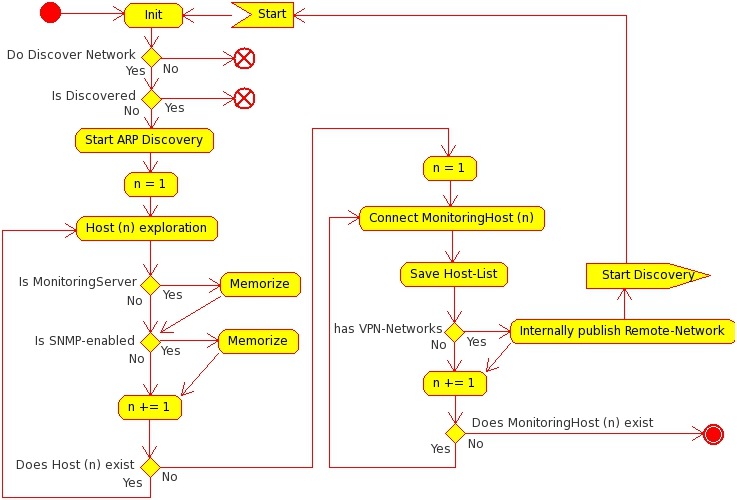
\includegraphics[width=\linewidth]{images/theorie/AutoDiscovery}
  \caption[Ablauf zum Suchen von neuen Systemen in einem Netzwerk]{Automatische Suche nach allen Hosts im internen wie auch in entfernten Netzwerken. Dieses wird nur neu ausgelesen, sofern dies nicht schon gemacht worden ist. Dadurch wird verhindert, dass ein Netzwerk von mehreren \"Uberwachungsservern nacheinander oder gleichzeitig ausgelesen wird.}
  \label{fig:discovery-ablauf}
\end{figure}


\subsection{Fazit: Problemfall Ger\"ateerkennung} \label{sec:theorie-discovery-fazit}
In gr\"osseren Netzwerken oder Verb\"unden verschiedener Netzwerke ist eine reine manuelle Konfiguration sehr aufw\"andig und daher praktisch unm\"oglich. Eine reine automatische Erkennung von Ger\"aten bietet jedoch eine zu geringe M\"oglichkeit zur individuellen Konfiguration der einzelnen Systeme.

Eine Mischform aus einer manuellen und einer automatischen Konfiguration ist die einfachste und komfortabelste L\"osung zur Einrichtung eines \"Uberwachungsnetzwerkes. Dabei k\"onnen einzelne Systeme jederzeit manuell in ein Netzwerk eingebunden, umkonfiguriert und ausgeschlossen werden, jedoch kann in einem Netzwerk auch automatisch nach neuen Komponenten gesucht werden.

Das zu implementierende System muss also \"uber beide M\"oglichkeiten verf\"ugen. Zum einen k\"onnen die \"Uberwachungsserver sowie verschiedene Komponenten in einem Netzwerk manuell konfiguriert werden, jedoch besteht auch die M\"oglichkeit dieses automatisch zu untersuchen. Dabei muss auf den \"Uberwachungsservern manuell definiert werden, welche Netzwerke miteinander verbunden sind und welche von diesen automatisch untersucht werden sollen, respektive welche nicht\footnote{\label{foot:theorie-discovery-fazit}Der Ausschluss eines Netzwerkes macht zum Beispiel bei Root-Servern Sinn, welche bei einem Hoster direkt im Internet sind, dort jedoch nicht das komplette Netzwerk, sondern nur eben der eine (oder mehrere) Server \"uberwacht werden soll.}. Diese Konfiguration muss nicht auf jedem \"Uberwachungsserver in jedem Netzwerk gemacht werden. Es reicht dabei aus, wenn diese Konfiguration auf einem einzelnen Server gemacht wird, denn die Konfiguration wird automatisch auf alle bekannten \"Uberwachungsserver \"ubertragen (siehe \ref{sec:theorie-config-fazit}).


%%%%%%%%%%%%%%%%%%%%%%%%%%%%%%%%%%%%%%%%%%%%%%%%%%%%%%%%%%%%%%%%%%%%%%%%%%%%%%%%%%%%%%%%%%%%%%%%%%%%%%%%%%%%%%%%%%%%%%%%%%%%%%%%%%%%%%%%%
\section{Problemfall Konfiguration} \label{sec:theorie-config}
Die verschiedenen \"Uberwachungsserver k\"onnen, wie zum Beispiel unter \ref{sec:theorie-discovery-fazit} definiert, unterschiedlich und individuell konfiguriert werden. Das gesamte \"Uberwachungsnetzwerk kann also auf jedem X-Beliebigen \"Uberwachungsserver ver\"andert werden. Diese Konfiguration muss anschliessend nicht nur auf alle anderen Systeme \"ubertragen sondern auch abgeglichen werden.

\subsection{M\"oglichkeiten zur Konfigurationsspeicherung} \label{sec:theorie-config-variants}
Grunds\"atzlich kann zwischen einer globalen und einer individuellen Konfiguration unterschieden werden.

\subsubsection{Global zusammengefasste Konfiguration} \label{sec:theorie-config-variants-global}
Eine M\"oglichkeit besteht darin, dass jeder \"Uberwachungsserver jeweils die komplette Konfiguration speichert.

Der Vorteil bei dieser Art der Speicherung liegt in der einfachen Handhabung, denn es gibt nur eine einzige Konfiguration. Diese kann auf einem beliebigen System angepasst und anschliessend 1:1 an alle anderen Server wieder ausgeliefert werden.

Nachteilig an dieser Variante ist jedoch, dass bei einem grossen \"Uberwachungsnetzwerk die Konfiguration relativ gross werden kann. Je nach Anzahl Komponenten und Diensten wird diese Art der Konfiguration relativ schnell komplex und wahrscheinlich fast nicht mehr \"uberschaubar (ohne entsprechende Konfigurations-Hilfen/-Programme).

\subsubsection{Individuelle Konfiguration} \label{sec:theorie-config-variants-individual}
Die zweite M\"oglichkeit beinhaltet eine individuelle Konfiguration auf jedem einzelnen System. Jeder \"Uberwachungsserver besitzt somit nur seine jeweilige Konfiguration und weiss dadurch auch nur, was er zu \"uberwachen hat. Die restlichen Systeme und Netzwerke sind ihm nicht bekannt.

Der Vorteil dieser Variante liegt eindeutig in der Konfigurationsgr\"osse, welche relativ klein und pro System sehr \"ubersichtlich ist.

Der grosse Nachteil liegt im Management der verschiedenen Konfigurationen. F\"ur einen globalen \"Uberblick \"uber die komplette Konfiguration, oder auch nur dar\"uber, welche Server den einen Dienst auf einem Server \"uberwacht, muss die komplette Konfiguration aus dem ganzen \"Uberwachungsnetzwerk zusammengesucht, kombiniert und ausgewertet werden. F\"ur diesen Vorgang m\"ussen nicht nur alle \"Uberwachungsserver im eigenen Netzwerk bekannt sein und abgefragt werden sondern auch alle in allen anderen Netzwerken.

\subsection{Fazit: Problemfall Konfiguration} \label{sec:theorie-config-fazit}
Das zu entwickelnde \"Uberwachungssystem soll sich automatisch, autonom und vor allem hochverf\"ugbar \"uberwachen. Eine Voraussetzung ist somit, eine schnelle und vor allem unkomplizierte Auswahl von verschiedenen \"Uberwachungspartnern. Dies kann nur mit einer global zusammengefassten Konfiguration erreicht werden.

Die Performance der einzelnen Systeme ist auch eine Voraussetzung, gerade im Bereich der Hochverf\"ugbarkeit. Dieser Aspekt kann jedoch nur durch eine individuelle lokale Konfiguration gew\"ahrleistet werden.

Durch diese Voraussetzungen kommt nur eine Kombination der beiden Varianten in Frage. Zus\"atzlich wird die Konfiguration noch in verschiedene Bereiche aufgeteilt, welche separiert gespeichert und abgefragt werden k\"onnen.

\subsubsection{Konfiguration der Netzwerke} \label{sec:theorie-config-fazit-network}
Die verschiedenen Netzwerke sowie die Verbindungen zwischen diesen werden in einer globalen, netzwerk\"ubergreifenden Konfiguration gespeichert. Dadurch wissen immer alle \"Uberwachungssysteme, welche anderen Netzwerke \"uberwacht werden und wie auf diese zugegriffen wird. Diese Konfiguration beinhaltet nur die Netzwerke und deren Daten zur Fragmentierung, Angaben ob das Netzwerk automatisch untersucht werden darf (siehe \ref{sec:theorie-discovery-fazit}), Verbindungsdaten f\"ur die Verbindungen (siehe \ref{sec:theorie-nat-fazit}) sowie eventuelle weitere Daten, welche auf den Netzwerken definiert werden m\"ussen. Dies k\"onnen zum Beispiel Dienste sein, welche von ausserhalb erreichbar sein m\"ussen, etc.

Diese globale Konfiguration ist nicht als eine zentrale Datenbank zu sehen sondern als eine Konfiguration, welche auf jedem System gleich ist. Bei einer Anpassung wird somit jedes System mit der neuen Konfiguration versehen und nicht nur das betroffene System.

\subsubsection{Konfiguration der Hosts und Systeme} \label{sec:theorie-config-fazit-systems}
Die verf\"ugbaren Hosts sowie deren Dienste, die \"uberwacht werden sollen, sind jeweils nur Netzwerkintern als globale Konfiguration vorhanden. Diese Konfiguration wird jeweils bei einer automatischen Ger\"ateerkennung und auch einer manuellen Anpassung neu geschrieben und verteilt. Auch diese globale Konfiguration ist nicht eine zentrale Datenbank, sondern grunds\"atzlich einfach auf jedem System gleich.

Interne Dienste, wie beispielsweise die \"Uberwachung des Arbeitsspeichers oder der Systemlast, werden gleich behandelt wie externe Dienste. Alle internen Dienste sollten ebenfalls \"uber einen SNMP-Dienst von extern abrufbar sein.

Durch diese Konfiguration weiss jedes System, was auf welchem anderen System laufen muss, was f\"ur Probleme auftreten k\"onnen und was bei einem Fehler passieren soll.

\subsubsection{Konfiguration der \"Uberwachungspartner} \label{sec:theorie-config-fazit-partner}
Die Auswahl der \"Uberwachungspartner muss automatisch und autonom erfolgen (siehe \ref{sec:theorie-fragmentierung}). Die Konfiguration, welches System welche Hosts und Dienste \"uberwacht, wird jeweils auf den Systemen und nicht global gespeichert. Somit kann schnell eruiert werden, wann was wo \"uberwacht werden soll, ohne zuerst andere Systeme an zu fragen, ob dies noch der Fall ist oder ob sich etwas ge\"andert hat.

Diese Konfiguration wird automatisch erstellt, gewartet und gel\"oscht. Sie kann nicht manuell bearbeitet werden.


%%%%%%%%%%%%%%%%%%%%%%%%%%%%%%%%%%%%%%%%%%%%%%%%%%%%%%%%%%%%%%%%%%%%%%%%%%%%%%%%%%%%%%%%%%%%%%%%%%%%%%%%%%%%%%%%%%%%%%%%%%%%%%%%%%%%%%%%%
\section{Problemfall Host-Fragmentierung} \label{sec:theorie-fragmentierung}
Sind alle Systeme gefunden und untersucht, muss in einem n\"achsten Schritt festgelegt werden, welche \"Uberwachungsserver welche anderen Systeme \"uberwachen sollen.

Die Grundfrage "`Wer \"uberwacht wen?"' beinhaltet folgende weiteren Fragestellungen, welche bei den verschiedenen Methoden zur Hostfragmentierung gekl\"art werden m\"ussen:
\begin{itemize}
 \item Werden die Dienste nur Netzwerk intern \"uberwacht oder auch von externen Systemen?
 \item Wie viele Server \"uberwachen einen einzelnen Dienst auf einem System?
 \item K\"onnen verschiedene \"Uberwachungen zu unterschiedlichen Zeitpunkten gemacht werden?
 \item Darf ein Server denjenigen \"uberwachen, welcher einen seiner Dienste \"uberwacht?
 \item \"Uberwacht ein Server nur einen einzelnen Server oder \"uberwacht er verschiedene Systeme?
 \item \"Uberwacht ein Server alle Dienste eines anderen oder nur einzelne?
\end{itemize}

In Kapitel \ref{sec:theorie-nat-fazit} wurde die Verbindung zwischen unterschiedlichen Netzwerken behandelt. Dadurch ist die erste Frage schon abgehandelt. In jedem Netzwerk steht mindestens ein \"Uberwachungsserver, welcher eine Verbindung in die anderen Netzwerke hat. Diese Server sind daf\"ur zust\"andig, die entfernten Netzwerke zu \"uberwachen. Das beinhaltet nicht nur die Erreichbarkeit, sondern auch die \"Uberwachung aller Dienste, welche als "`von extern zu \"uberwachen"' konfiguriert worden sind (siehe Kapitel \ref{sec:theorie-config-fazit-network}).

Die Frage nach der Anzahl Server, welche einen einzelnen Dienst auf einem System \"uberwachen, kann einfach beantwortet werden: Durch die Definition einer hochverf\"ugbaren \"Uberwachung, sollte ein Dienst, wenn m\"oglich, immer von mehreren anderen Systemen \"uberwacht werden und nicht nur von einem einzelnen. F\"allt ein System aus, wird die \"Uberwachung somit immer noch von mindestens einem anderen Ger\"at durchgef\"uhrt.

Die restlichen Fragen gehen in den Bereich der Performance und der Lastverteilung.

\subsection{Lastverteilung} \label{sec:theorie-frag-last}
Die Systemlast sollte, gerade da es sich um eine hochverf\"ugbare \"Uberwachung handelt und die Server nicht zus\"atzlich belastet werden sollen, m\"oglichst gering sein und somit eine hohe Performance aufweisen. Die zu \"uberwachenden Dienste m\"ussen also m\"oglichst gleichverteilt auf alle internen \"Uberwachungsserver verteilt werden. Durch diese Gleichverteilung kann davon ausgegangen werden, dass jeder \"Uberwachungsserver eine \"ahnliche, zus\"atzliche Grundlast aufweist. Mit der Formel
\begin{equation}
 L = {X \times N}
\label{eq:theorie-frag-nonshared}
\end{equation}
kann berechnet werden, was f\"ur eine zus\"atzliche Last $L$ ein \"Uberwachungsserver verkraften muss, wenn je nur ein einzelner Dienst von allen Servern \"uberwacht wird. Dabei wird f\"ur $X$ die Last des jeweiligen Dienstes und f\"ur $N$ die Anzahl \"uberwachter Server genommen.

\begin{table}[ht]
 \centering
 \begin{tabular}{r|c|c|c|c}
   & HTTP (50) & SMTP(10) & ICMP (5) & POP3 (30) \\
  \hline
  Server A & x & x & x & x \\
  \hline
  Server B & x &   & x &   \\
  \hline
  Server C &   &   & x &   \\
  \hline
  Server D & x & x & x & x \\
  \hline
  Server E & x &   & x &   \\
  \hline
  Total    & 4 & 2 & 5 & 2
 \end{tabular}
 \caption[Zu \"uberwachende Server und Dienste]{Beispiel: Verschiedene Server mit unterschiedlichen Diensten, die \"uberwacht werden sollen. In Klammern ein Dummy-Wert zur Berechnung, welcher die zus\"atzliche "`Last"' einer \"Uberwachung angibt. Eine HTTP-Dienst\"uberwachung mit Result-Auswertung braucht mehr Resourcen als eine einfacher ICMP-EchoRequest.}
 \label{tbl:theorie-frag-hosts}
\end{table}

\begin{table}[ht]
 \centering
 \begin{tabular}{r|c|c|c|c|c}
   & HTTP (50) & SMTP(10) & ICMP (5) & POP3 (30) & Zus\"atzliche Last \\
  \hline
  Server A & 4 &   &   &   & 200 \\
  \hline
  Server B &   & 2 &   &   & 20 \\
  \hline
  Server C &   &   & 5 &   & 25 \\
  \hline
  Server D &   &   &   & 2 & 60 \\
  \hline
  Server E &   &   &   &   & 0
 \end{tabular}
 \caption[Lastenvergleich, wenn gruppiert nach Dienst \"uberwacht wird]{Beispiel: Jeder Server \"ubernimmt die \"Uberwachung von einem einzelnen Dienst. In Klammern ein Dummy-Wert zur Berechnung, welcher die zus\"atzliche "`Last"' einer \"Uberwachung angibt. Jeder Server hat somit eine stark unterschiedliche Zusatzlast, mit Ausnahme von Server E, welcher nicht weiter belastet wird. Problematisch sind nicht nur die unterschidlichen Lasten, sondern auch dass die Server ihre eigenen Dienste \"uberwachen m\"ussen.}
 \label{tbl:theorie-frag-nonshared}
\end{table}

Damit die zus\"atzliche Grundlast m\"oglichst gleichverteilt auf allen Systemen ist, sollte eine m\"oglichst gemischte Dienst\"uberwachung gew\"ahlt werden. Die verschiedenen Dienst\"uberwachungen weisen wahrscheinlich unterschiedliche Lasten in der Verarbeitung auf, denn bei den einen Diensten muss lediglich die Erreichbarkeit gekl\"art werden, bei anderen m\"ussen eventuell komplexe Stringmanipulationen oder verschiedene Sende- und Empfangs-Aktionen durchgef\"uhrt werden. Durch die Definition, dass ein \"Uberwachungsserver unterschiedliche Dienste \"uberwacht, kann also sichergestellt werden, dass eine Lastverteilung stattfindet. Mit der Formel
\begin{equation}
 L = \sum_{i=0}^{N} {X_i}
\label{eq:theorie-frag-shared}
\end{equation}
kann diese Zusatzlast $L$, welche ein Server verkraften muss, berechnet werden. Dabei ist $i$ ein Z\"ahler von $0$ bis zur Anzahl Dienste $N$ und $X_i$ die jeweilige Last des aktuellen Dienstes.

F\"ur eine genaue Berechnung und optimale Lastverteilung ist es dabei notwendig, dass die Summe der Last der Dienste gleichm\"assig auf alle Server verteilt werden kann. Es m\"usste also "`$AnzahlDienste \mod AnzahlServer = 0$"' gegeben sein, um eine optimale Verteilung zu gew\"ahrleisten. Diese Definition sagt aus, dass jedem Server gleich viele Dienste zugewiesen werden k\"onnen, die Berechnung $AnzahlDienste \over AnzahlServer$ also keinen Rest ergibt - Wobei bei dieser Definition die Last der Dienste nicht beachtet wird. Ein Vergleich zwischen den zwei Varianten ist, basierend auf den Daten aus Tabelle \ref{tbl:theorie-frag-hosts}, in den Tabellen \ref{tbl:theorie-frag-nonshared} und \ref{tbl:theorie-frag-shared} zu sehen.

\begin{table}[ht]
 \centering
 \begin{tabular}{r|c|c|c|c|c}
   & HTTP (50) & SMTP(10) & ICMP (5) & POP3 (30) & Zus\"atzliche Last \\
  \hline
  Server A & 1 &   & 1 &   & 55 \\
  \hline
  Server B & 1 & 1 & 1 &   & 65 \\
  \hline
  Server C & 1 &   & 1 & 1 & 85 \\
  \hline
  Server D & 1 &   & 1 &   & 55 \\
  \hline
  Server E &   & 1 & 1 & 1 & 45
 \end{tabular}
 \caption[Lastenvergleich, wenn die Dienste auf alle Server aufgeteilt werden]{Beispiel: Die 13 Dienste werden auf die verschiedenen Server aufgeteilt. Somit werden die Lasten nahezu gleich auf alle Server verteilt.\newline}
 \label{tbl:theorie-frag-shared}
\end{table}

Eine andere M\"oglichkeit besteht darin, dass ein \"Uberwachungsserver jeweils alle Dienste von einem oder von mehreren anderen Systemen \"uberwacht. Die dabei anfallende Last kann mit der Formel
\begin{equation}
L = \sum_{k=0}^{M} \left( \sum_{i=0}^{N} {X_{k_i}} \right)
\label{eq:theorie-frag-sysshared}
\end{equation}
berechnet werden, wobei $M$ die Anzahl der Server, $N$ die Anzahl der Dienste auf dem Server $M_k$ und $X_{k_i}$ die Last des Dienstes $X_i$ auf dem aktuellen Server ist. Tabelle \ref{tbl:theorie-frag-sysshared} zeigt die Systemlasten, welche bei einer solchen \"Uberwachung anfallen w\"urden.

\begin{table}[ht]
 \centering
 \begin{tabular}{r|c|c|c|c|c}
   & HTTP (50) & SMTP(10) & ICMP (5) & POP3 (30) & Total Last \\
  \hline
  Server A & 1 & 1 & 1 & 1 & 95 \\
  \hline
  Server B & 1 &   & 1 &   & 55 \\
  \hline
  Server C &   &   & 1 &   & 5 \\
  \hline
  Server D & 1 & 1 & 1 & 1 & 95 \\
  \hline
  Server E & 1 &   & 1 &   & 55
 \end{tabular}
 \caption[Lastenvergleich, wenn alle Dienste eines Servers \"uberwacht werden]{Beispiel: Alle Dienste auf einem System werden von einem Server \"uberwacht. Die Tabelle zeigt die Lasten, welche beim \"Uberwachungs-Server anfallen w\"urden.}
 \label{tbl:theorie-frag-sysshared}
\end{table}

Da ein System meistens mehrere andere Rechner \"uberwacht, muss bei dieser Variante darauf geachtet werden, dass die Auswahl der unterschiedlichen Systeme zu einer gleichverteilten Last f\"uhrt. Die zus\"atzliche Last sollte also bei jedem \"Uberwachungsserver um den Mittelwert aller Lasten liegen. Um dies zu erreichen, kann ein einfacher Algorithmus (siehe Codeblock \ref{alg:theorie-frag-mittelwert}) angewendet werden.
\begin{figure}[H]
 \lstset{language=Pascal}
 \begin{lstlisting}[mathescape,literate={<=}{{$\leq$}}1{>=}{{$\geq$}}1{<>}{{$\neq$}}1,label=alg:theorie-frag-mittelwert,caption={[Gleicheverteile Lastenverteilung der Dienste auf Server]Mit diesem Algorithmus werden alle zu \"uberwachenden Dienste und Server gleichverteilt auf alle \"Uberwachungsserver verteilt. Die Server liegen dabei als Liste $hosts \Rightarrow [h_1, h_2, ..., h_k]$ vor. Die Hosts werden der Last nach sortiert und anschliessend immer die beiden \"aussersten Systeme (also der Last-Intensivste und -Extensivste) einem Host zugewiesen.}]
if numMonitor >= 1 and numMonitor <= length(hosts)-1 then
  result {}
end

if count(hosts) = 2 then
  result { $h_1$:[$h_2$], $h_2$:[$h_1$] }
end

back = {}
intensiveLoad = floor(numMonitor / 2)
extensiveLoad = intensiveLoad

if numMonitor modulo 2 <> 0 then
  extensiveLoad = intensiveLoad + 1
end

hosts = sort_ascending_by_load(hosts)
monitoredHosts = []

for host in hosts do
  if length(monitoredHosts) = length(hosts) then
    monitoredHosts = []
  end

  x = 0
  while length(back[host]) <> intensiveLoad do
    if length(monitoredHosts) = length(hosts) break
    if hosts[x] <> host and hosts[x] not in monitoredHosts then
      add hosts[x] to back[host]
      add hosts[x] to monitoredHosts
    end
    x += 1
  end

  x = length(hosts) - 1
  while length(back[host]) <> intensiveLoad + extensiveLoad do
    if length(monitoredHosts) = length(hosts) break
    if hosts[x] <> host and hosts[x] not in monitoredHosts then
      add hosts[x] to back[host]
      add hosts[x] to monitoredHosts
    end
    x -= 1
  end
end

result back
 \end{lstlisting}
\end{figure}


\subsection{Anzahl \"Uberwachungspartner} \label{sec:theorie-fragmentierung-numhosts}
Durch die Anzahl der \"Uberwachungspartner wird nicht nur die Grundlast, welche auf den Servern anf\"allt, definiert, sondern auch die zus\"atzliche Last im Netzwerk, sowie der gesamte Vernetzungsplan. Durch die definierte Autonomit\"at der \"Uberwachungsstrategie, sollte also nicht eine fixe Anzahl an Verbindungen vorgegeben werden, sondern diese sollte automatisch berechnet werden.

Eine M\"oglichkeit best\"unde darin, dass einfach jeder Rechner jeden anderen \"uberwachen w\"urde. Dies w\"are jedoch nicht nur performancetechnisch Unsinn, sondern auch administrativ. F\"allt beispielsweise in einem Netzwerk mit 100 Rechnern ein System aus, w\"urden 99 andere Systeme das bemerken und m\"ussten untereinander ausmachen, wer denn nun den Alert ausl\"ost und versendet.

Es muss also ein Algorithmus entworfen/gefunden werden, welcher die ideale Anzahl an Verbindungen zwischen verschiedenen Knotenpunkten herstellt. Die Distanz zwischen zwei Punkten, respektive zwischen zwei Systemen kann dabei vernachl\"assigt werden, denn die Latenzen in einem internen Netzwerk m\"ussen sowieso als sehr klein angenommen werden\footnote{\label{foot:theorie-frag-latenzen}Sind die Latenzen in einem internen Netzwerk, also z.B. einem Geb\"aude, schlecht, stimmt entweder etwas an der Verkabelung nicht, das Netzwerk ist \"uberlastet oder es werden alte Komponenten eingesetzt, welche mit der Last nicht zurecht kommen.}.

In der Informatik schon lange eingesetzte und bew\"ahrte Techniken bei Kommunikationsintensiven Abl\"aufen sind die Hypercube-Algorithmen\footnote{Danke an dieser Stelle f\"ur den Hinweis auf die Hypercubes an Herr Dr. Frank Moehle.}. Die nachfolgenden Formeln sowie die Definitionen der Hamming-Distanz sind in vielen Fachliteraturen und im Internet verf\"ugbar, zum Beispiel im Dokument von Hans Walser: Der n-dimensionale Hyperw\"urfel \cite{hypercube}. Dieses Dokument diente als Grundlage f\"ur den Aufbau des grundlegenden Verst\"andnisses der Hyperw\"urfel.

Ein Hypercube, auch Hyperw\"urfel genannt, stellt grunds\"atzlich ein Netzwerk aus Knoten und Verbindungen dar (siehe Abbildung \ref{fig:hyper-sample} im Anhang). Der Einsatz der Hypercubes im Bereich des Hypercomputing oder auch Clustering r\"uhrt daher, dass grunds\"atzlich von jedem Knoten des Hypercubes eine Verbindung zu jedem anderen Knoten besteht. Die Anzahl an Verbindungen bleibt dabei jedoch \"uberschaubar, da nicht einfach jeder Knoten mit jedem anderen verbunden wird. Es bestehen aber auch nicht zu wenige Verbindungen, so dass das Fehlen eines Systems nicht zu einem Totalausfall f\"uhrt.

Bei einem Hypercube werden alle Systeme je einem Knoten zugewiesen. Die Distanz zwischen zwei Systemen ist im Optimalfall $1$, im schlimmsten Fall gleich der Dimension $n$ des Hypercubes\footnote{\label{foot:hypercube-dimension}Die Dimension beim Hypercube ergibt sich aus der Anzahl von Systemen, die \"uberwacht werden m\"ussen siehe Abbildung \ref{fig:hyper-sample} im Anhang}. Diese Distanz wird auch \textit{Hamming-Distanz}\footnote{\label{foot:hypercube-hamming}Die \textit{Hamming-Distanz} findet ihren Ursprung bei Richard Wesley Hamming, welcher durch den Hamming-Code eine Selbst-Korrigierende \"Ubermittlungsmethode entwickelte.} genannt, entsprechend werden im Hypercube auch die verschiedenen Ecken nummeriert und verbunden (siehe Abbildung \ref{fig:hyper-hamming-num} im Anhang).

Zur Bestimmung der Dimension des Hypercubes muss die Anzahl der Systeme bekannt sein. Die Anzahl Ecken in einem Hypercube wird definiert durch $2^n$, wobei $n$ die Dimension ist. Es muss also die n\"achst h\"ohere Zweierpotenz gefunden werden, um die Dimension des Hypercubes zu bestimmen (siehe Codeblock \ref{alg:theorie-hypercube-dimension}). Basierend auf der Dimension k\"onnen anschliessend alle weiteren Daten berechnet werden.

\begin{figure}[H]
 \lstset{language=[ANSI]C}
 \begin{lstlisting}[label=alg:theorie-hypercube-dimension,caption={[N\"achst h\"ohere Zweierpotenz finden]Algorithmus zum Auffinden der n\"achst h\"oheren Zweierpotenz zur Dimensionsbestimmung eines Hypercubes anhand der Anzahl Systeme. Die Schlaufe "`schiebt"' dabei die 1 in der bin\"aren Darstellung so lange nach links bis die Potenz gr\"osser oder gleich der Anzahl Systeme ist.}]
// bin: 0000 0001
power = 1
if (numHosts > 1) {
  while (power < numHosts) {
    // Shift left as long as power is less than numHosts
    // bin: 0000 0010, 0000 0100, 0000 1000, ...
    power <<= 1
  }
}
return power
 \end{lstlisting}
\end{figure}

Die Anzahl \"Uberwachungspartner bei einem Hypercube ist immer gleich der Dimension. Somit kann durch den Algorithmus in Codeblock \ref{alg:theorie-frag-mittelwert} bestimmt werden, welche Systeme welche anderen \"uberwachen. Dies jedoch nur unter der Voraussetzung, dass jedes System das \"uberwacht wird, ebenfalls ein \"Uberwachungsserver ist. Das kann aber nicht als Voraussetzung gegeben werden, denn in einem Netzwerk werden oft Ger\"ate eingesetzt, welche sich zwar \"uberwachen lassen, selber jedoch nicht in der Lage sind, andere Systeme zu \"uberwachen - geschweige denn es zulassen, Software nach zu installieren, welche diese Funktionalit\"at \"ubernehmen w\"urde.

Eine M\"oglichkeit, dieses Problem zu umgehen w\"are, eine spezielle Anordnung der Nodes im Hypercube. Dies w\"urde eine relative Verkomplizierung des Algorithmus nach sich ziehen, denn bei jeder Platzierung m\"ussten alle Nachbarknoten angeschaut werden und auf die \"Uberwachungsf\"ahigkeit untersucht werden.

Eine weitaus einfachere M\"oglichkeit ist, den Hypercube nur mit den \"Uberwachungsservern als Knoten zu erstellen. Die restlichen Systeme werden anschliessend einfach harmonisch auf alle \"Uberwachungsserver aufgeteilt.

Durch folgende Vorgehensweise kann schnell und einfach eine \"Uberwachung basierend auf einem Hypercube aufgebaut werden:
\begin{enumerate}
 \item Dimension des Hypercubes anhand aller \"Uberwachungsserver feststellen
 \item Hypercube mit allen \"Uberwachungsservern erstellen
 \item \"Uberwachungspartner festlegen, die Anzahl ist gleich der Dimension
 \item Die restlichen Systeme auf alle \"Uberwachungsserver aufteilen
\end{enumerate}

\subsection{Leere Knoten im Hypercube} \label{sec:theorie-fragmentierung-spof}
Die Vernetzung aller \"Uberwachungsserver mittels einem Hypercube ist eine schnelle und nicht sehr rechenintensive Angelegenheit. Ein Hypercube, welcher basierend auf einer Anzahl Hosts aufgebaut wird, welche keine Zweierpotenz ist, weist aber eine grosse Unsch\"onheit auf: leere Knoten. Gerade wenn ein Hypercube mit vielen Systemen erstellt wird, nimmt die Wahrscheinlichkeit zu, dass leere Knoten in einem Hypercube vorhanden sind.

Im schlimmsten Fall kann ein Node durch diese leeren Knoten so abgeschirmt werden, dass dieser nur Verbindungen zu leeren Knoten aufweist. Eine Illustrierung dieses Problems wird in Abbildung \ref{fig:hyper-spof-9hosts} gezeigt. Ein Hypercube, der basierend auf 9 Systemen aufgebaut wird, muss in der Dimension $d=4$ erstellt werden. Das bedeutet, dass es total $2^4 - 9 = 16 - 9 = 7$ leere Knoten gibt und jeder Knoten 4 Verbindungen aufweist. Im extremsten Fall k\"onnen so bis zu vier Nodes komplett abgeschirmt sein. Bei einer Verwendung des Hypercubes zur Gew\"ahrleistung von Verbindungen von jedem Node im Netzwerk zu jedem anderen, kann dies zu schwerwiegenden Problemen f\"uhren.

\begin{figure}[ht]
  \centering
  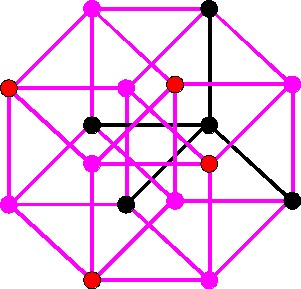
\includegraphics[width=0.5\linewidth]{images/theorie/hyper-spof-9hosts}
  \caption[Ein Hypercube der vierten Dimension]{Ein Hypercube der vierten Dimension mit 9 Hosts (schwarz, rot) weist 7 leere Knoten auf (magenta). Bei einer ungl\"ucklichen Zuweisung der Nodes k\"onnen so bis zu vier Systeme ohne Verbindung sein (rot).}
  \label{fig:hyper-spof-9hosts}
\end{figure}

Beim Aufbauen eines Hypercubes muss also immer darauf geachtet werden, dass die Nodes nicht willk\"urlich im Hypercube verteilt werden, sondern dass diese der Reihe nach aufgef\"ullt werden. Dadurch kann gew\"ahrleistet werden, dass jeder Knoten mindestens eine Verbindung aufweist.



%%%%%%%%%%%%%%%%%%%%%%%%%%%%%%%%%%%%%%%%%%%%%%%%%%%%%%%%%%%%%%%%%%%%%%%%%%%%%%%%%%%%%%%%%%%%%%%%%%%%%%%%%%%%%%%%%%%%%%%%%%%%%%%%%%%%%%%%%
\section{Problemfall ALERT-\"Ubermittlung} \label{sec:theorie-alert}
Wird von einem System ein Fehler entdeckt, muss dies je nach Konfiguration einer entsprechenden Person oder Stelle gemeldet werden. Die Problematik liegt nun darin, dass ein System, respektive Dienst, von mehreren anderen Systemen zu unterschiedlichen Zeitpunkten \"uberwacht wird. Eine Meldung sollte aber wenn m\"oglich nur einmal versendet werden und nicht von jedem \"Uberwachungssystem aus, welches den Fehler bemerkt.

\subsection{Zentrale Meldestelle} \label{sec:theorie-alert-zentral}
Eine M\"oglichkeit diese mehrfache Alert-Auslieferung in den Griff zu bekommen, w\"are eine zentrale Meldestelle. Jedes Problem, welches entdeckt wird, wird umgehend dieser zentralen Stelle gemeldet. Eine Meldung muss dabei mindestens die Zeit der \"Uberwachung, den Meldungs-Typen sowie allf\"allige Daten beinhalten. In regelm\"assigen Abst\"anden werden alle gespeicherten und nicht versendeten Meldungen ausgelesen, gruppiert und verschickt.

Die Gruppierung der Meldungen nach dem Zeitrahmen und Meldungs-Typ hat den Hintergrund, dass die verschiedenen \"Uberwachungssysteme die Pr\"ufungen zwar nicht zum gleichen Zeitpunkt daf\"ur aber im gleichen Intervall\footnote{Ein System soll zum Beispiel alle 5 Sekunden mit einem ECHO-Request auf Anwesenheit gepr\"uft werden. Dieses Interval kann prinzipiell gew\"ahrleistet werden, nicht jedoch dass jedes System die gleiche Pr\"ufung in der gleichen (Nano/Mili)Sekunde ausf\"uhrt.} ausf\"uhren. Werden nun alle Nachrichten innerhalb eines solchen Intervalls ausgelesen (unter Beachtung des Systems und Dienstes), kann theoretisch ausgeschlossen werden, dass der gleiche Vorfall mehrfach gemeldet wird.

Der Vorteil einer solchen zentralen Instanz w\"are klar die einfache Bearbeitung aller Fehler. Der Nachteil liegt jedoch in der Definition und der Auslegung des gesamten \"Uberwachungs-Systems. Da das komplette System "`hochverf\"ugbar"' sein muss, w\"are eine einzelne wenn auch nur Netzwerk interne Alert-Instanz ein Widerspruch sowie eine Fehlerquelle. Funktioniert diese zentrale Instanz nicht oder ist diese nicht erreichbar, k\"onnen aus dem gesamten Netzwerk keine Fehler gemeldet werden.

\subsection{Hochverf\"ugbare Alert-\"Ubermittlung} \label{sec:theorie-alert-ha}
Um dem Paradigma der Hochverf\"ugbarkeit gerecht zu werden, sollte prinzipiell jeder \"Uberwachungsserver in der Lage sein, einen Fehler eigenst\"andig zu melden. In diesem Szenario gibt es zur Vermeidung von mehrfachen Meldungen grunds\"atzlich zwei M\"oglichkeiten\footnote{Diese zwei M\"oglichkeiten beschreiben die Basisfunktionalit\"at - Kombinationen und Verfeinerungen, etc. sind m\"oglich, werden aber nicht als weitere M\"oglichkeiten gelistet.}:

\begin{itemize}
 \item[POLL:] Wird ein Fehler entdeckt, m\"ussen alle anderen Systeme, welche das gleiche System und den gleichen Dienst \"uberwachen, angefragt werden, ob dieser Fehler innerhalb der letzten X Zeiteinheiten schon gemeldet worden ist. Ist dies nicht der Fall, wird eine Meldung gesendet und der Status gespeichert.
 \item[PUSH:] Wird ein Fehler entdeckt, m\"ussen alle anderen Systeme benachrichtigt werden, dass dieser Fehler zum Zeitpunkt X gemeldet worden ist. Entdeckt ein anderes System den gleichen Fehler, kann es durch diese interne Liste pr\"ufen, ob der gefundene Fehler innerhalb der letzten X Zeiteinheiten schon gemeldet worden ist oder nicht.
\end{itemize}

Bei beiden m\"oglichen Szenarien besteht die Gefahr, dass das Netzwerk unn\"otigerweise belastet respektive \"uberflutet wird. Jedes System setzt nach der offiziellen \"Uberwachung noch weitere Anfragen an alle anderen Systeme ab. Die Anzahl der Anfragen\footnote{Wenn $n$ Systeme gleichzeitig an alle $n-1$ anderen Systeme eine Anfrage stellen, sind gleichzeitig $n*(n-1)$ Requests auf dem Netzwerk} kann sich dadurch auf ein Maximum von $n*(n-1)$ kumulieren.

Die Anfragen und Antworten werden wahrscheinlich relativ kleine Datenpakete sein. Die heutigen internen Netzwerke sind rasend schnell, jedoch sollen mit der angestrebten L\"osung auch Systeme mit einer schwachen Leitung\footnote{Zum Beispiel ein einzelnes externes System, welches lediglich \"uber eine GSM-Verbindung verf\"ugt} und auch stark frequentierte und ausgelastete Netzwerke angesprochen und \"uberwacht werden k\"onnen. Bei der zu implementierenden L\"osung muss dieser Punkt unbedingt beachtet werden.

\subsection{Fazit: Problemfall ALERT-\"Ubermittlung} \label{sec:theorie-alert-fazit}
Das zu entwickelnde System muss hochverf\"ugbar sein, aus diesem Grund kommt eine zentrale Alert-Meldestelle, welche ausfallen k\"onnte, nicht in Frage. Jedes System muss in der Lage sein, eine Meldung zu versenden sowie eigenst\"andig zu eruieren, ob eine Meldung versendet werden soll und kann. Die einzelnen Systeme m\"ussen sich also gegenseitig sperren k\"onnen, was durch ein Mutex-Verfahren\footnote{Ein Mutex, englisch f\"ur \textbf{mut}ual \textbf{ex}clusion (wechselseitiger Ausschluss), verhindert, das nebenl\"aufige Prozesse oder Threads gleichzeitig auf gleiche Datenstrukturen zugreifen und diese ver\"andern.} realisiert wird. Ein einzelnes System muss also alle anderen Systeme mit einem \textit{Lock}\footnote{\textit{Locking} bedeutet \textit{Sperren}, also das beabsichtigte verhindern der Ausf\"uhrung einer Aktion, Funktion, Dateizugriff, etc.} versehen k\"onnen. Dabei wird basierend auf dem ausgefallenen Dienst, dem System und der Ausfallzeit auf jedem System ein \textit{Semaphor}\footnote{Ein Semaphor beschreibt in der Informatiok eine Datenstruktur zur Steuerung des ausschliessenden Zugriffes. Ein Semaphor beinhaltet alle Daten, welche genutzt werden, um den Ausf\"uhrungszeitpunkt zu bestimmen.} erstellt, welcher dieses Locking steuert. Durch die Zeit des Fehlers sowie eines konfigurierten Timeouts kann so jedes System feststellen, ob ein Fehler gemeldet werden soll oder nicht.

Ein m\"oglicher Ablauf einer \"Uberwachung und Alert-\"Ubermittlung ist in Abbildung \ref{fig:alert-sample} zu sehen. Bei dieser Visualisierung wird sowohl die PUSH- wie auch die POLL-Methode gezeigt. Bei einem POLL wird jedes mal beim Auftreten eines Fehlers jedes andere System angefragt, wann und ob der Fehler schon versandt worden ist. Jedes System gibt bei der Polling-Methode eine Semaphor zur\"uck, anhand welcher dies dann gepr\"uft werden kann. Rein rechnerisch kann die Anzahl Verbindungen, welche bei der POLL-Methode anfallen, durch
\begin{equation}
C = e \times (n-1)
\label{eq:theorie-alert-last}
\end{equation}
berechnet werden. Wobei $C$ die Anzahl an Verbindungen, $e$ die Anzahl der gleichen Fehler und $n$ die Anzahl Server beschreibt. Diese Formel kann auch f\"ur eine Standard-Implementation der PUSH-Methode verwendet werden, denn auch bei dieser muss bei jedem auftreten eines Fehlers eine Semaphor an jedes System gesendet werden.

\begin{figure}[h]
  \centering
  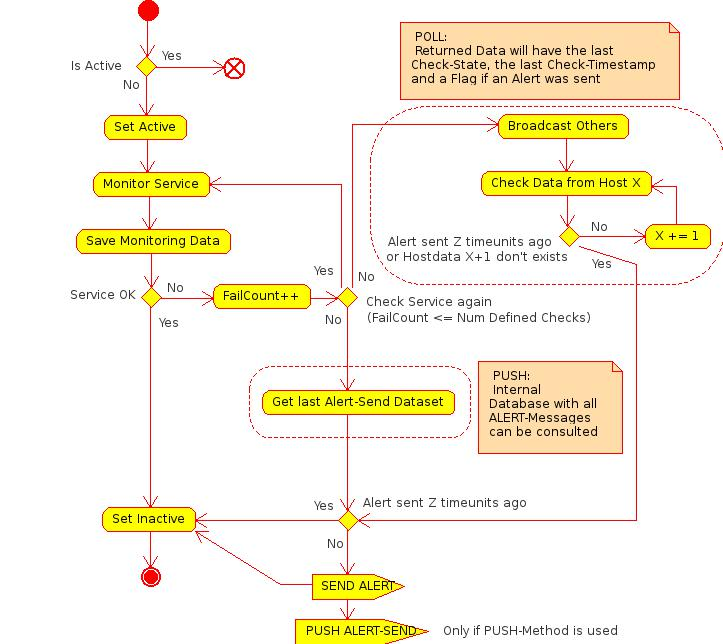
\includegraphics[width=0.9\linewidth]{images/theorie/AlertSend}
  \caption[Ablauf einer \"Uberwachung und Alarmmeldung]{Eine \"Uberwachung wird nur dann gestartet, wenn aktuell keine aktiv am laufen ist. Schl\"agt ein Test fehl, kann dieser erneut durchgef\"uhrt werden. Wenn alle Tests fehlgeschlagen sind, werden entweder alle anderen Systeme angefragt (POLL) und anhand deren Daten entschieden ob ein Meldung versendet werden muss oder nicht oder es werden die Internen Daten des letzten PUSH-Requests dazu verwendet.}
  \label{fig:alert-sample}
\end{figure}

Um die optimalste Anzahl an Verbindungen zu erlangen, muss die Anzahl an Fehlern $e$ in der obigen Formel \ref{eq:theorie-alert-last} reduziert oder gar weggelassen werden. Dieser Ansatz wurde in der PUSH-Methode in Abbildung \ref{fig:alert-sample} verwendet: Die Semaphor wird nur dann gesendet, wenn auch ein Alert verschickt wird. Das setzt voraus, dass jedes System alle Meldungen empf\"angt und intern speichert, denn nur so k\"onnen die Systeme die Semaphor f\"ur das Locking der Alerts nutzen. Semaphoren, welche durch die angegebene Zeiteinheit das Alerting nicht mehr blockieren, k\"onnen aus dem Speicher entfernt werden, so dass neue Fehler wieder gemeldet werden k\"onnen. Unter Ber\"ucksichtigung dieser Definition kann die Verbindungsanzahl durch \begin{equation}
C = (n-1)
\label{eq:theorie-alert-optimal}
\end{equation}
berechnet werden.

Ist ein System, durch einen Netzwerkausfall oder \"ahnliches, komplett isoliert\footnote{Ein System kann komplett isoliert sein durch fehlende oder falsche Routen, ausgesteckte oder defekte Netzwerkkabel, defekte Netzwerkkarten, uvm.} von allen anderen \"Uberwachungssystemen, kann ein Semaphor weder angefragt noch empfangen werden. Ist dies der Fall, und das Alerting ist nicht durch einen Lock gesperrt, wird der Fehler von dem System grunds\"atzlich gemeldet. In den meisten F\"allen f\"uhrt dies aber zu keinem doppelten oder mehrfachen Alert-Meldungs aufkommen, denn durch den Netzwerkfehler sind meistens auch die Alert-Nachrichten-Server (SMTP, SMS, etc.) nicht erreichbar. Durch die vernetzte Struktur wird das isolierte System aber von den anderen Servern erkannt und gemeldet.

Durch dieses Mutex-Verfahren kann bei den Alert-Meldungen komplett auf ein kompliziertes Transaktions-System verzichtet werden. Die Kombination des Push von Semaphoren und dem Locking reicht in den meisten F\"allen dazu aus, ein mehrfaches versenden von Alert-Meldungen zu unterbinden. Ausgeschlossen werden kann dies jedoch nicht, da der Empfangszeiptunkt der Semaphor nicht garantiert werden kann. Es besteht bei dieser Variante also die M\"oglichkeit, dass eine Semaphor zum Zeitpunkt $X$ gesendet und von einem System erst zum Zeitpunkt $X + 2$ empfangen wird. Pr\"uft nun das zweite System zum Zeitpunkt $X+1$ ob das senden erlaubt ist, weiss es nichts vom Sendeprozess des ersten Systems und sendet ebenfalls einen Alert. Durch eine Wartezeit zwischen dem Senden der Semaphore und dem Senden des Alerts sowie einer erneuten Pr\"ufen, kann dieses Problem umgangen werden. Wird bei der zweiten Pr\"ufung eine Semaphore gefunden, also ein Sendeprozess eines anderen Systems, erh\"allt jeweils das System mit dem kleineren Zeitstempel, also das erste System, den Vortritt zum Senden des Alerts.


%%%%%%%%%%%%%%%%%%%%%%%%%%%%%%%%%%%%%%%%%%%%%%%%%%%%%%%%%%%%%%%%%%%%%%%%%%%%%%%%%%%%%%%%%%%%%%%%%%%%%%%%%%%%%%%%%%%%%%%%%%%%%%%%%%%%%%%%%
\section{Techniken zur Nachrichten\"ubermittlung} \label{sec:theorie-msg}
Zur \"Ubermittlung von Nachrichten, sei dies durch einen Push- oder einen Pop-Request\footnote{\label{foot:push-pop}Ein Push-Request ist eine unaufgeforderte Zusendung von Daten; ein Pop-Request hingegen ist das aktive Anfragen von Daten}, gibt es nicht nur verschiedene Techniken sondern auch verschiedene Technologien. Zur \"Ubermittlung von \"Uberwachungsdaten haben sich dabei nachfolgende Standards etabliert, welche bei der zu implementierenden Software auch eingesetzt werden sollen.

\subsection{SNMP} \label{sec:theorie-snmp}
Das \textit{Simple Network Management Protocol} (SNMP) ist ein standardisiertes Netzwerkprotokoll zur \"Uberwachung und Steuerung von Netzwerkkomponenten. Das Protokoll wurde so festgelegt, dass prinzipiell jedes netzwerkf\"ahige Ger\"at in die \"Uberwachung aufgenommen werden kann. Dabei wird nicht nur der Aufbau der Datenpakete definiert, sondern ebenso der komplette Kommunikationsablauf. Um die Grundlast auf dem Netzwerk so gering wie m\"oglich zu halten, wird das Verbindungslose Protokoll UDP genutzt.

SNMP kennt insgesamt sechs verschiedene Paketarten. Die drei verschiedenen GET-Pakete\footnote{\label{foot:snmp-get-pkgs}SNMP kennt ein GET-Paket zum Anfragen von Daten, das GETNEXT-Paket um einen nachfolgenden Datensatz z.B. aus einer Tabelle aus zu lesen sowie das GETBULK-Paket zum Abrufen von mehreren Datens\"atzen} werden jeweils von einem Manager\footnote{Bei SNMP wird der Server mit Manager und der Client mit Agent beschrieben.} an einen Agenten gesendet, worauf dieser mit einem RESPONSE-Paket antwortet. Das SET-Paket wird genutzt um Parameter auf einem Agenten zu ver\"andern. Das TRAP-Paket schlussendlich ist ein einfacher Push-Request. Es wird also unaufgefordert ein Paket von einem Agenten an einen Manager gesendet. Traps werden dazu genutzt, um einen Manager dar\"uber zu informieren, dass ein Ereignis aufgetreten ist. Der Agent kann dabei nicht feststellen, ob das Paket beim Manager angekommen und verarbeitet worden ist, denn ein TRAP-Paket kann nicht durch ein RESPONSE-Paket best\"atigt werden.

SNMP definiert zwar den Aufbau der Datenpakete (siehe Anhang \ref{fig:snmp-packet}), nicht jedoch die Daten selbst, welche \"ubertragen werden. Die Daten und Werte, welche von einem Ger\"at ausgelesen werden k\"onnen, werden als "`Managed Object"' \"ubertragen. Diese MOs sind durch eine \texttt{Management Information Base} (MIB)\footnote{\label{foot:snmp-mib}Die MIB, definiert in RFC-1155\cite{rfc1155} (siehe auch RFC-4293\cite{rfc4293}, RFC-4022\cite{rfc4022}, RFC-4113\cite{rfc4113}), beinhaltet keine Daten sondern den Aufbau eines "`Managed Objects"', welches verwendet wird um Daten zu versenden/empfangen.} definiert. Die Basis jedes MIB ist der \texttt{Object Identifier} (OID)\footnote{\label{foot:snmp-oid}Eine OID sollte eine Weltweit eindeutige Identifikation sein, um Verwechslungen zu vermeiden. Firmen k\"onnen bei der IANA (Internet Assigned Numbers Authority, \url{http://www.iana.org/}) kostenlos eigene MIB-Module unterhalb "`iso.org.dod.internet.private.enterprise"' beantragen (\url{http://pen.iana.org/pen/PenApplication.page}). Unterhalb dieses Zweiges k\"onnen anschliessend eigene OIDs definiert werden.} sowie die Definition der unterschiedlichen Datenfelder. Diese Datenfelder weisen nicht nur einen Namen auf, sondern unterliegen auch einem Datentyp. Datentypen k\"onnen einfache Zahlen oder Texte sein, jedoch auch vordefinierte Muster wie zum Beispiel eine IPv4-Adresse (siehe Codeblock \ref{code:mib-ipAddress} im Anhang).

Aktuell sind verschiedene Versionen von SNMP verf\"ugbar und im Einsatz. SNMPv1 wurde 1988 definiert und setzte den Fokus nicht gross auf die Datensicherheit. Aus diesem Grund wurden verschiedene SNMPv2 Versionen definiert, welche alle unterschiedliche Sicherheits- und Datenkonzepte aufweisen. Die am meisten verwendete Version ist SNMPv2-community (SNMPv2c). Die Sicherheit basiert bei SNMPv2c auf so genannten "`Communities"', bei welchen definiert werden kann, dass z.B. bei \texttt{PUBLIC} nur gelesen, bei \texttt{PRIVATE} jedoch zus\"atzlich auch geschrieben werden darf. Eine Sicherheitsfunktion wie ein Passwort gibt es dabei nicht. Es kann zwar ein komplizierter Community-Name definiert werden, da SNMPv2c aber nicht verschl\"usselt wird, bringt auch das keinen wirklichen Schutz.

Die Versionen SNMPv1 bis SNMPv2c bieten also weder eine gute Verschl\"usselung noch eine sichere M\"oglichkeiten zur Authentifizierung. Aus diesem Grund wurde im Dezember 2002 die Spezifikation von SNMPv3\footnote{\label{foot:snmpv3-rfc}SNMPv3 wird in folgenden RFCs definiert: RFC-3410\cite{rfc3410}, RFC-3411\cite{rfc3411}, RFC-3412\cite{rfc3412}, RFC-3413\cite{rfc3413}, RFC-3414\cite{rfc3414}, RFC-3415\cite{rfc3415}, RFC-3416\cite{rfc3416}, RFC-3417\cite{rfc3417}, RFC-3418\cite{rfc3418}} ver\"offentlicht, welche Benutzer- und Ansichts basierende Zugriffsbeschr\"ankungen sowie andere Sicherheitsmechanismen beinhaltet. Gerade wegen diesen neuen Sicherheitsfunktionen, wie zum Beispiel der Schl\"usselverwaltung, ist SNMPv3 noch nicht sehr verbreitet.

\subsubsection{Fazit: SNMP} \label{sec:theorie-snmp-fazit}
Trotz gravierender sicherheits bezogener M\"angel der Versionen SNMPv1 bis SNMPv2c ist SNMP dennoch eine schnelle und einfache sowie gut erweiterbare Technologie zur Abfrage und \"Ubermittlung von einfachen Datens\"atzen. Sofern die Sicherheit keine grosse Rolle spielt, k\"onnen diese SNMP-Versionen ohne Bedenken eingesetzt werden. Zur \"Ubertragung von kritischen Daten muss entweder SNMPv3 in einer verschl\"usselten Variante oder SNMPv2c/SNMPv3 \"uber eine verschl\"usselte Verbindung respektive \"uber ein komplett abgeschirmtes Management-Netzwerk verwendet werden.

SNMP kann genutzt werden, wenn Daten von einem System auf ein anderes \"ubertragen werden sollen. So kann SNMP zum Beispiel gut f\"ur eine Leistungs\"uberwachung genutzt werden, nicht jedoch f\"ur die Funktionspr\"ufung eines Webservices oder anderen Dienstes wie SMTP, POP3, etc.


\subsection{IPMI} \label{sec:theorie-msg-ipmi}
Der \textit{Intelligent Platform Management Interface} (IPMI) Standard wurde von verschiedenen Hardware-Herstellern entwickelt zur einfachen Wartung und Verwaltung von Hardware. Die Betriebssystem unabh\"angigen Schnittstellen erlauben es zudem, automatische Berichte \"uber allf\"allige Probleme zu versenden. Sie k\"onnen entweder \"uber eine serielle Schnittstelle oder auch \"uber das lokale Netzwerk genutzt werden. IPMI funktioniert sowohl w\"ahrend dem laufenden Betrieb, jedoch auch wenn dieses im Standby oder ausgeschaltet ist. Die einzige Voraussetzung ist eine Betriebsspannung auf den Komponenten.

Das Herzst\"uck von einem IPMI Ger\"at ist der \texttt{Baseboard Management Controller} (BMC)\footnote{\label{foot:ipmi-bmc}Auf den meisten heutigen Server-Boards ist bereits ein BMC verbaut, was die \"Uberwachung mittels IPMI sehr kosteng\"unstig und einfach macht}. Dieser Controller ist ein spezieller Mikrocontroller, an welchen alle daf\"ur ausgelegte Hardware angeschlossen werden kann\footnote{\label{foot:ipmi-bmc-smbus}Die Hardware muss \"uber einen SMBus verf\"ugen. Dies ist ein zweiadriger Bus mit maximal 100 kbit/s und basiert auf dem $I^2C$-Serialbus von Philips und ist abw\"artskompatibel zu diesem.}. Wird mit dem BMC \"uber das Netzwerk kommuniziert, kann optional eine Verschl\"usselung verwendet werden. Bei einer seriellen Verbindung wird grunds\"atzlich angenommen, dass die Verbindung sicher ist. F\"ur den Verbindungsaufbau wird jedoch in jedem Fall ein Passwort ben\"otigt.

\subsubsection{Fazit: IPMI} \label{sec:theorie-msg-ipmi-fazit}
IPMI ist grunds\"atzlich ein Management-Tool f\"ur Server und nicht ein Protokoll zur Daten\"ubertragung. Beispielsweise kann IPMI dazu genutzt werden, einen Server aus der Ferne zu analysieren, neu zu starten, den Startvorgang zu beobachten, etc. Daf\"ur muss das System aber \"uber die notwendige Hardware verf\"ugen und entsprechend konfiguriert sein.

Durch verschiedene Tools wie \textit{IPMItool}\cite{IPMItool} oder \textit{OpenIPMI}\cite{OpenIPMI} wird die Administration sowie der Zugriff auf ein IPMI-Systeme stark vereinfacht und kann auch automatisiert werden.

Bei der zu implementierenden Software kann angedacht werden, dass IPMI als zus\"atzliche Datenabfrage zur Auswahl steht.


\subsection{Andere Formate} \label{sec:theorie-msg-other}
Je nach Art der Pr\"ufung, sind eventuell andere Formate notwendig. Soll ein Service auf einem Webserver auf Funktionalit\"at gepr\"uft werden, kann nicht SNMP verwendet werden. Die Anfrage an den Dienst muss mittels HTTP \"uber TCP gemacht und die Antwort anschliessend entsprechend ausgewertet werden. Das selbe gilt f\"ur DNS-Pr\"ufungen, Mailserver-Tests und andere.

\subsection{Fazit: Andere Formate} \label{sec:theorie-msg-other-fazit}
Die Art der Daten\"ubermittlung darf bei dem zu entwickelnden System nicht eingeschr\"ankt werden. Das System soll durch Plugins nicht nur erweiterbar sein, sondern es sollen auch verschiedene Dienste und Services gepr\"uft werden k\"onnen. Die Art und das Format der Daten bei einer \"Uberwachung darf nicht eingeschr\"ankt werden.


%%%%%%%%%%%%%%%%%%%%%%%%%%%%%%%%%%%%%%%%%%%%%%%%%%%%%%%%%%%%%%%%%%%%%%%%%%%%%%%%%%%%%%%%%%%%%%%%%%%%%%%%%%%%%%%%%%%%%%%%%%%%%%%%%%%%%%%%%
\section{Techniken zur Alert-\"Ubermittlung} \label{sec:theorie-alertsend}
Je nach Schweregrad der Meldung muss eine solche schnell und umgehend einer verantwortlichen Person oder Stelle zugestellt werden. Dies setzt voraus, dass eine Nachricht \"uber verschiedene Kan\"ale \"ubermittelt werden kann, welche ebenfalls unterschiedlich priorisiert werden k\"onnen.

\subsection{EMail} \label{sec:theorie-alert-email}
EMail ist ein relativ unsicheres Medium zur Alert-\"Ubermittlung. Zum einen muss das System eine Verbindung mit einem EMail-Server besitzen, zum anderen muss der Empf\"anger auch vor dem Computer sitzen und regelm\"assig das entsprechende Postfach pr\"ufen.

Ein Vorteil von EMail ist sicherlich, dass alle Daten von einem Test direkt \"ubermittelt werden k\"onnen. Voraussetzung ist, dass der EMail-Server funktioniert und eine Verbindung mit diesem hergestellt werden kann. Der Fehler darf somit weder etwas mit dem Netzwerk noch mit der Internetverbindung oder dem EMail-Server zu tun haben.

Eine M\"oglichkeit w\"are, das EMail direkt vom System aus an den Empf\"anger-Mailserver zu senden, ohne Umweg \"uber einen internen/externen Mailserver. Durch die heutzutage eingesetzten Spam- und Virenfilter, treten dabei wahrscheinlich mehr Probleme auf als verhindert werden. Viele Mailserver blocken den ersten Zustellversuch\footnote{Beim Graylisting wird jeweils ein Zustellversuch geloggt und das erste mal geblockt. Erst der zweite Versuch vom gleichen Absender, an den gleichen Empf\"anger \"uber den gleichen Server wird dann erlaubt. Somit kommt ein EMail vielfach erst mit einer Verz\"ogerung von einigen Minuten oder Stunden beim Empf\"anger an.}, lassen unbekannte oder dynamische Absender erst gar nicht durch\footnote{Durch Realtime-Blacklists (RBL) werden dynamische Absender und bekannte Spamnetzwerke gesperrt}, verlangsamen absichtlich den Datenversand\footnote{Durch Tarpitting werden Verbindungen k\"unstlich verlangsamt um zu schauen ob die Gegenstelle ein richtiger Mailserver ist und kein Spamhost, welcher keine Zeit hat da er viele Nachrichten versenden muss} oder blocken Systeme, welche keine Mailserver sind, komplett\footnote{Teilweise werden Verbindungen zu den Absendern oder den Reverse-DNS Eintr\"agen aufgebaut um zu pr\"ufen ob dort ein richtiger Mailserver ist}.

\subsection{Fazit: EMail} \label{sec:theorie-alert-email-fazit}
Die Meldungszustellung \"uber EMail sollte grunds\"atzlich nur f\"ur Informative Zwecke verwendet werden und nicht f\"ur hoch kritische Nachrichten. EMail ist nicht nur langsam, sondern es kann auch nicht gew\"ahrleistet werden, dass eine Meldung wirklich zugestellt wird - vorallem nicht in einem angemessenen Zeitrahmen.

\subsection{SMS-Nachricht} \label{sec:theorie-alert-sms}
Das Senden und Empfangen von SMS-Nachrichten ist eine schnelle und einfache Art der Nachrichtenzustellung. Eine SMS ist beschr\"ankt in der Anzahl Zeichen, welche versendet werden k\"onnen. Somit k\"onnte beim Auftauchen eines Fehlers lediglich eine kurze Beschreibung oder eine Zusammenfassung versendet werden.

Die Nachrichtenzustellung per SMS hat drei gravierende Nachteile:
\begin{itemize}
 \item Ein System muss entweder mit einer GSM-Komponente ausgestattet werden, welche den Versand der SMS \"ubernimmt oder es muss ein Online-Dienst zum Versenden in Anspruch genommen werden.
 \item Die Zustellung einer SMS wird von den Mobile-Com-Firmen nicht garantiert, denn die Sprachdienste sind auf dem GSM-Netzwerk h\"oher priorisiert als Datendienste, es sei denn, man hat spezielle Vertr\"age, welche aber nur Beh\"orden und Notfalldienste bekommen \cite{tannenbaum}.
 \item Ist der Empf\"anger nicht erreichbar, kann nicht gew\"ahrleistet werden, dass die Nachricht wirklich zugestellt wird oder wurde \cite{tannenbaum}.
\end{itemize}

Weiter zu bedenken ist, dass bei vielen Dienstleistern das Versenden einer SMS Kosten verursacht. Es kann passieren, dass bei einem Fehler oder einer falsch konfigurierten Regel eine Unmenge an Nachrichten versendet werden, welche somit hohe Kosten verursachen.

\subsubsection{Fazit: SMS-Nachrichten} \label{sec:theorie-alert-sms-fazit}
Jedes System mit einer GSM-Komponente sowie mit einer g\"ultigen SIM-Karte und einem Vertrag aus zu statten, w\"urde nicht nur in einer kleinen sondern auch in einer grossen Konfiguration den Kostenrahmen sprengen. Eine M\"oglichkeit w\"are, pro Netzwerk nur einige Systeme mit einer GSM-Komponente aus zu statten. Zus\"atzlich sollte auch die Einbeziehung von einem oder mehreren Online-Services f\"ur den SMS-Versand genutzt werden k\"onnen.

Die Gew\"ahrleistung, dass eine Nachricht wirklich zugestellt wird, kann nicht gegeben werden\footnote{Bei SMS kann nur durch eine Statusabfrage gepr\"uft werden, ob eine Nachricht dem Empf\"anger zugestellt worden ist oder nicht \cite{tannenbaum}.}. SMS sollte also immer in Kombination mit einer anderen Variante verwendet werden: Die Verantwortliche Person wird per SMS und per EMail, welches alle gesammelten Daten beinhaltet, \"uber den Fehler informiert.

\subsection{Paging} \label{sec:theorie-alert-paging}
Paging, oder auch Funkmeldeempf\"anger (FME), wird vielfach zur Nachrichten\"ubermittlung und Alarmierung eingesetzt. Der grosse Vorteil eines Pagers gegen\"uber einem GSM-Ger\"at ist, dass ein Pager durch die unterschiedliche Technik nicht nur in abgelegenen Bereichen\footnote{Die Abdeckung der Schweiz durch die SWISSPHONE liegt beim Paging bei ca. 99\%, wie auch die Netzabdeckung von GSM durch die Swisscom, Orange oder Sunrise. Bei GSM gibt es jedoch viele kleine Inseln, welche auch in urbanen Gegenden zu einer schwachen oder gar keiner Abdeckung f\"uhren k\"onnen.}, in welchen ein Mobiltelefon keinen Empfang hat, funktioniert, sondern auch, dass die Zustellung einer Paging-Nachricht prinzipiell gew\"ahrleistet werden kann. Aus diesem Grund setzen immer noch viele Notfalldienste wie Feuerwehr und Rettungsdienst auf diese Technik und nicht auf GSM.

Ein FME kann prinzipiell mit einem Funkger\"at verglichen werden, welches dauernd auf Empfang ist. Unterliegen die empfangenen Daten einem Muster, also einer Reihe von T\"onen, werden alle nachfolgenden Daten weiterverarbeitet und angezeigt. Die Digitalen Melde Empf\"anger (DME und POCSAC) arbeiten auf einer h\"oheren Frequenz als die FME\footnote{Ein FME ist rein Analog, es werden also T\"one \"ubertragen welche ausgewertet werden. Ein DME hingegen kann auf dem 2-Meter Band arbeiten, welches Analoge Signale nicht mehr geeignet ist. Die POCSAG-Ger\"ate arbeiten in einer noch h\"oheren Frequenz}. Die DME-Ger\"ate k\"onnen zudem in verschiedenen Ausbaustufen genutzt werden. Die einfachste Stufe, die DME-I Ger\"ate, besitzen lediglich vordefinierte Texte, welche mittels einer gesendeten Bitfolge aufgerufen werden k\"onnen. Die zweite Ausbaustufe, die DME-II Ger\"ate, sind zudem noch in der Lage, Freitextnachrichten (\"ahnlich einer SMS) zu empfangen. Die h\"ochste Ausbaustufe bieten DME-III Ger\"ate, welche den empfangenen Text anhand eines integrierten Lexikons in Sprache \"ubersetzen und wiedergeben.

Die kommenden Generationen werden wohl \"uber das TETRA-Netzwerk agieren, welches \"ahnlich wie das GSM-Netzwerk auf Zellen basiert und somit nicht nur eine "`Gespr\"achsweitergabe"' sondern auch eine Lokalisierung erlaubt\footnote{Ein Alert k\"onnte somit derjenigen Person zugestellt werden, welche geographisch gesehen am n\"achsten bei dem fehlerhaften System ist.}. Vorteil der TETRA-basierenden Ger\"ate ist die M\"oglichkeit, auf eine Meldung reagieren zu k\"onnen. Dies ist bei den aktuellen FME-, DME- und POCSAG-Ger\"aten nur in Kombination mit einem weiteren Kommunikationskanal wie GSM m\"oglich. Der Nachteil der TETRA-Netzwerke ist aber der selbe wie bei GSM: Durch die Zellen k\"onnen wie bei GSM viele kleine Funkl\"ocher entstehen\footnote{Die Problematik der Funkl\"ocher m\"ussen aktuell diverse deutsche Stellen und St\"adte erfahren, welche eine Umstellung auf den POCSAC-Standard vollziehen ohne diesen ausf\"uhrlich getestet zu haben. Ein Beispiel hierzu ist die Stadt M\"unchen: \url{http://www.heise.de/security/meldung/Muenchen-mit-grossen-BOS-Digitalfunk-Loechern-1148126.html}}.

\subsubsection{Fazit: Paging} \label{sec:theorie-alert-paging-fazit}
Die Nachrichten\"ubermittlung \"uber ein DME- oder POCSAG-Ger\"at ist eine schnelle, einfache und vor allem zuverl\"assige M\"oglichkeit einen Alarm zu versenden. Obwohl die Netzabdeckung des Paging-Netzwerkes zahlenm\"assig ungef\"ahr gleich ist wie diejenige des GSM-Netzwerkes, gibt es dennoch weniger Funkl\"ocher, da das Paging-Netzwerk nicht auf verschiedene Frequenzen und unterschiedliche Zellen aufgeteilt ist. Das Paging-Netzwerk ist eine grosse Fl\"ache. Befindet man sich innerhalb dieser Fl\"ache, kann man eine Nachricht empfangen (\"ahnlich wie das ein Funkamateur macht).

Ein grosser Nachteil einer Paging-Nachricht ist jedoch die "`Nicht-\"Uberpr\"ufbarkeit"' der Zustellung. Auch das eigentliche Versenden einer Pager-Nachricht kann sich als schwer erweisen, denn diese werden in den meisten F\"allen direkt \"uber das Internet zum Netz-Anbieter gesendet und dann von diesem weiter verschickt. Ist die Internetanbindung also nicht vorhanden, kann kein Alarm ausgel\"ost werden.

Zudem kann auch die Kostenfalle zu einem Problem werden, wie schon bei SMS beschrieben.


\subsection{Andere M\"oglichkeiten} \label{sec:theorie-alert-other}
Neben den vorgestellten M\"oglichkeiten zur \"Ubermittlung von Meldungen, gibt es noch weitere Techniken f\"ur die gleiche Angelegenheit. So k\"onnen zum Beispiel alle Meldungen mittels einem SNMP-Trap an eine oder mehrere Stellen gesendet werden, welche diese dann auswerten und anzeigen. Wenn jedoch mehr Daten versendet werden sollen, k\"onnte dies auch \"uber eine einfache XML-Schnittstelle und HTTP erledigt werden oder \"uber eine einfache RS232-Schnittstelle (COM-Port), an welcher ein Display, eine Alarmzentrale, etc. angeschlossen ist.


\subsection{Fazit: Techniken zur Alert \"Ubermittlung} \label{sec:theorie-alert-fazit}
Die Alarmierung ist in den meisten F\"allen abh\"angig von einer funktionierenden Internet-Verbindung. Sei dies f\"ur eine EMail-Nachricht oder um den Paging-/SMS-Anbieter zu erreichen, welcher Nachrichten \"uber einen Webservice empfangen und versenden kann. Verschiedene Techniken wie SMS oder Paging w\"urden es auch erlauben, externe Hardware f\"ur den Versand zu nutzen. Ob diese Hardware nun an jedem \"Uberwachungssystem angeschlossen ist oder nur an einer zentralen Stelle im Netzwerk, darf bei der zu implementierenden L\"osung keine Rolle spielen.

Eine Alarmierungs-Technik sollte grunds\"atzlich \"uber eine Schnittstelle angesprochen und so erweitert werden k\"onnen. Dadurch k\"onnen verschiedene M\"oglichkeiten unterschiedlich genutzt werden. Sei dies nun eben, dass ein SMS mittels einem zentralen SMS-Gateway, einer RS232-Schnittstelle oder einem Webservice versendet werden soll. Bei der \"Uberwachungssoftware sollte prinzipiell nur gesagt werden, dass bei einem Alarm vom Typ XY, ein SMS versendet werden soll sowie zus\"atzlich ein EMail mit allen Daten. Die komplette Priorisierung, was genau bei einem Alarm vom Typ XY gemacht werden soll, wird in der jeweiligen Alarmierungs-Erweiterung definiert.


